\documentclass[a4j]{ujarticle}
\renewcommand{\baselinestretch}{0.85}
\usepackage[top=1.5cm, bottom=1.5cm, left=1.5cm, right=1.5cm]{geometry}
\usepackage{xcolor}
\usepackage[dvipdfmx]{graphicx, hyperref}
\usepackage{listings}
\usepackage{multirow}
\usepackage{siunitx}
\usepackage{subfig}
\usepackage{url}
\usepackage{listings}
\usepackage{caption,stackengine}

\colorlet{punct}{red!60!black}
\definecolor{background}{HTML}{EEEEEE}
\definecolor{delim}{RGB}{20,105,176}
\colorlet{numb}{magenta!60!black}

\newcommand{\Sref}[1]{\mbox{\ref{sec:#1}}}
\newcommand{\Tref}[1]{\mbox{表\ref{tab:#1}}}
\newcommand{\Eref}[1]{\mbox{式(\ref{eq:#1})}}
\newcommand{\Fref}[1]{\mbox{図\ref{fig:#1}}}
\renewcommand{\lstlistingname}{ソースコード}
\newcommand{\Lref}[1]{\mbox{ソースコード\ref{lst:#1}}}
\newcommand{\bhline}[1]{\noalign{\hrule height #1}}

\hypersetup{
	setpagesize=false,
	bookmarksnumbered=true,
	bookmarksopen=true,
	colorlinks=true,
	linkcolor=black,
	citecolor=black
}

\begin{document}
    \begin{flushright}
        MDLab GM資料\\
        22年7月12日(火)
    \end{flushright}

    \begin{center}
        {\Large	距離学習を導入したCenterNetによる\\腹部超音波画像からの肝腫瘍検出と分類}
    \end{center}

    \begin{flushright}
        {\large B4 原 英吾}\\
    \end{flushright}

    \section{研究背景および目的}
    \begin{figure}[h]
        \begin{minipage}{.59\textwidth}
            \begin{itemize}
                \item 背景
                \begin{itemize}
                    \item 器具の操作と診断を同時に行わなければならず高難易度
                    \item 肝臓は沈黙の臓器と呼ばれ初期には自覚症状がほとんどない
                    \begin{itemize}
                        \item 症状を自覚している時には重症化している場合が多い
                    \end{itemize}
                    \item 機械学習による診断のサポート
                    \begin{itemize}
                        \item 良性・悪性を見分けることが重要視される
                        \item \Fref{ex}の様に明らかなラベル不足\footnotemark[1]のある画像が存在する
                    \end{itemize}
                \end{itemize}
                \item 目的
                \begin{itemize}
                    \item 既存の研究を踏まえたモデルの精度向上
                    \begin{itemize}
                        \item 良性・悪性判別の高精度化
                    \end{itemize}
                    \item 超音波支援システムの開発
                    \begin{itemize}
                        \item 早期発見につながると良い
                    \end{itemize}
                \end{itemize}
            \end{itemize}
        \end{minipage}
        \begin{minipage}{.39\textwidth}
            \centering
            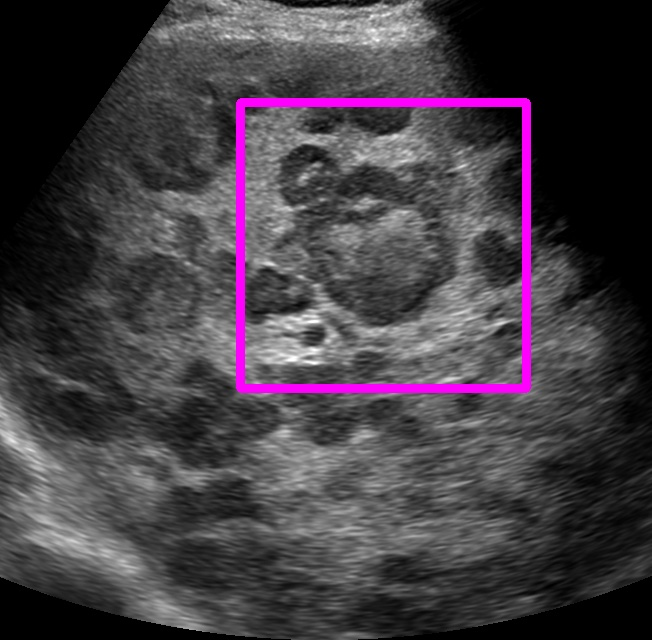
\includegraphics[width=.9\linewidth]{../fig/pseudo_a.png}
            \caption{ラベル不足のある診断画像例}
            \label{fig:ex}
        \end{minipage}
    \end{figure}

    \footnotetext[1]{今回は\Fref{ex}の様なアノテーションが不足しているものを指す}
    \addtocounter{footnote}{1}

    \section{これまでの研究のまとめ}
        \begin{itemize}
            \item データセット
            \begin{itemize}
                \item 国立研究開発法人日本医療研究開発機構(AMED)\footnote{\url{https://www.amed.go.jp/}}が提供している延べ8万枚に及ぶ以下のデータが付随
                \begin{itemize}
                    \item 腹部超音波画像,ROI
                    \item 年齢,性別
                \end{itemize}
                \begin{figure}[h]
                    \centering
                    \subfloat[性別毎の画像枚数]{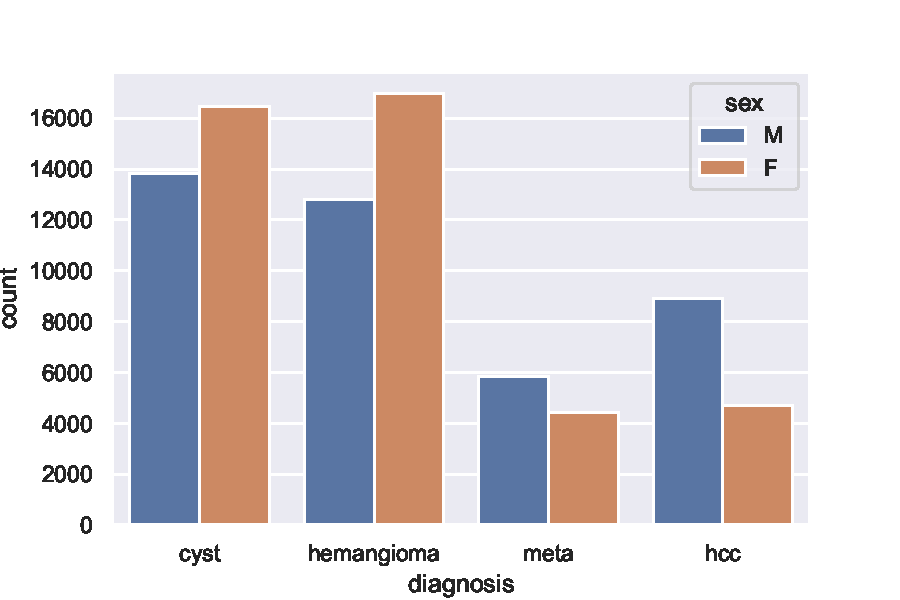
\includegraphics[width=.24\linewidth]{../fig/sex_a.pdf} \label{fig:sex}}
                    \subfloat[診断名毎の年齢分布]{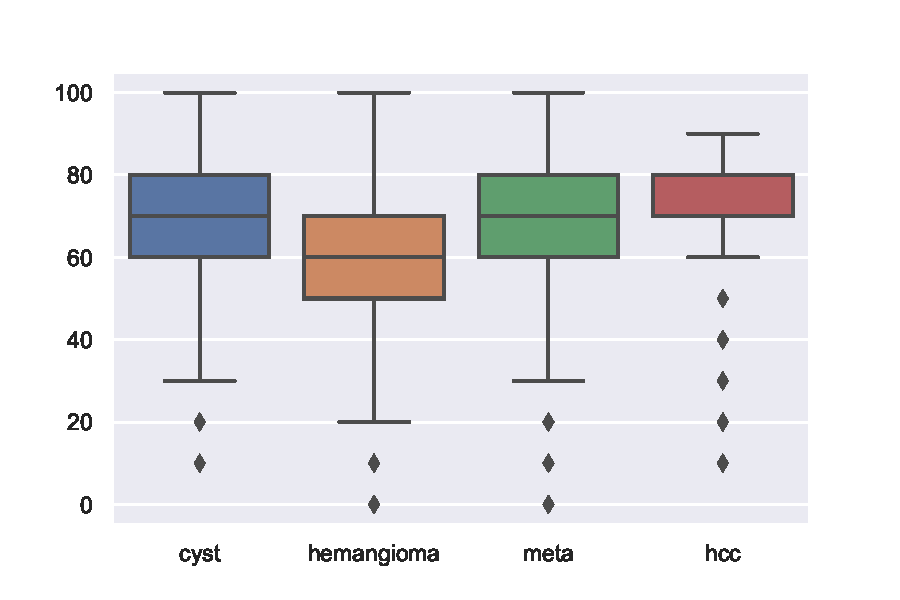
\includegraphics[width=.24\linewidth]{../fig/age_a.pdf} \label{fig:age}}
                    \subfloat[診断名毎の画像サイズの分布]{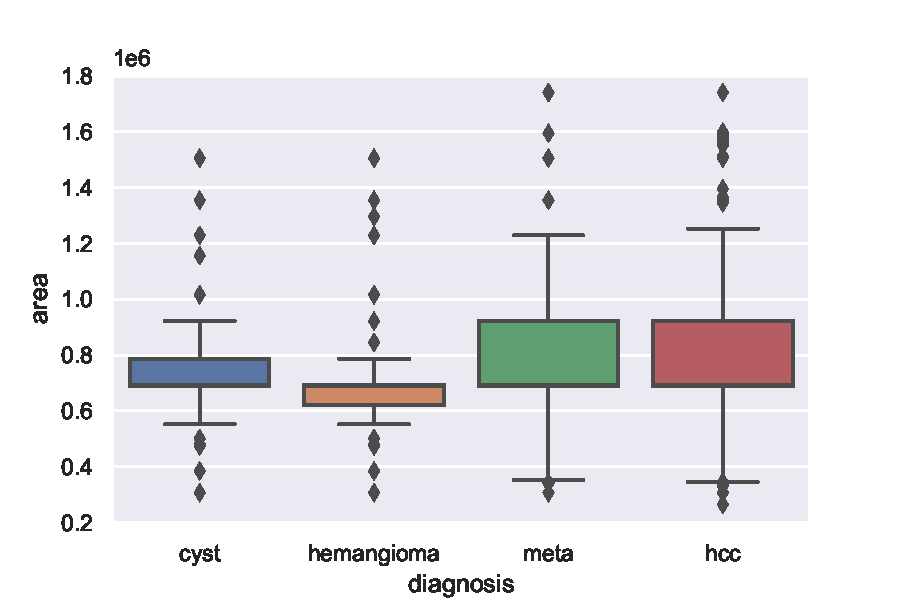
\includegraphics[width=.24\linewidth]{../fig/area_a.pdf} \label{fig:area}}
                    \subfloat[診断名毎のbboxの割合]{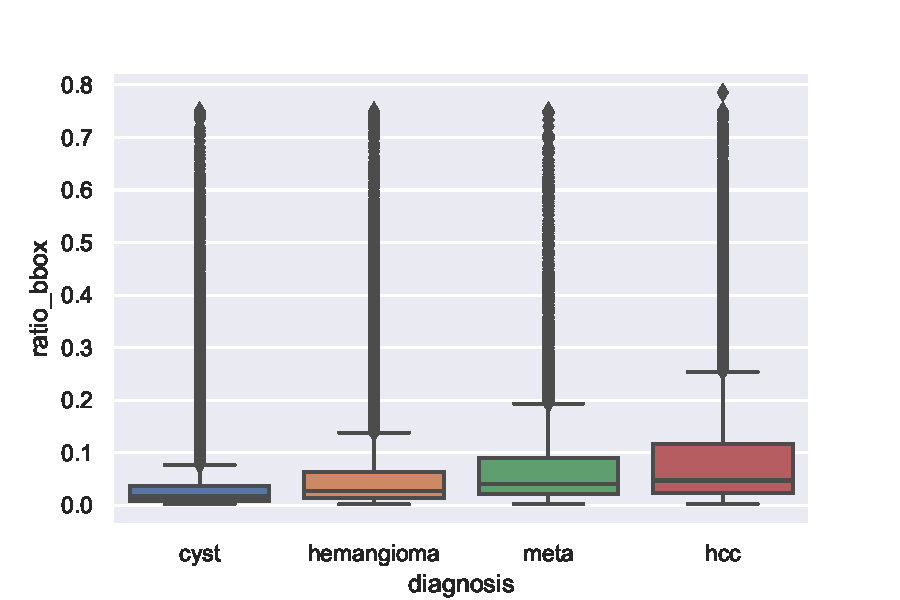
\includegraphics[width=.24\linewidth]{../fig/ratio_bbox_a.pdf} \label{fig:ratio}}
                    \caption{データセットにおけるデータの分布}
                \end{figure}
                \item 性別(\Fref{sex})
                \begin{itemize}
                    \item HCC(肝細胞癌)は男性が罹患しやすい
                    \begin{itemize}
                        \item 昔は男性の方が飲酒・タバコが多く癌に罹りやすかったという時代背景があるかもしれない
                    \end{itemize}
                    \item hemangioma(血管腫)は女性が罹患しやすい
                    \item Meta(転移性肝癌)は他の症状よりも少ない
                \end{itemize}
                \item 年齢(\Fref{age})
                \begin{itemize}
                    \item cyst(単純嚢胞),hemangioma(血管腫)の分布にははあまり特徴がない
                    \item hemangioma(血管腫)は比較的若年層でも罹患する
                    \item Meta(転移性肝癌)における0歳はラベルミスである可能性が高い
                    \item HCC(肝細胞癌)は比較的高齢者が罹患しやすい
                \end{itemize}
                \item 画像サイズ(\Fref{area})
                \begin{itemize}
                    \item hemangioma(血管腫)は比較的画像サイズが統一されている
                    \begin{itemize}
                        \item 腫瘍の大きさが血管に依存するためあまり偏りが生じていない?
                    \end{itemize}
                \end{itemize}
                \item bboxの画像に占める割合(\Fref{ratio})
                \begin{itemize}
                    \item cyst(単純嚢胞)は他の診断と比べてbboxの割合が低い($\frac{1}{2}$程度)である
                    \item HCC(肝細胞癌)は画像に占めるbboxの割合が高い
                \end{itemize}
            \end{itemize}
        \end{itemize}

        \begin{itemize}
            \item 症状毎の特徴を調査
            \begin{figure}[h]
                \centering
                \subfloat[cyst(単純嚢胞)]{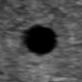
\includegraphics[width=.24\linewidth]{../fig/cyst.png} \label{fig:cyst}}
                \subfloat[HCC(肝細胞癌)]{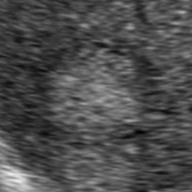
\includegraphics[width=.24\linewidth]{../fig/hcc.png} \label{fig:hcc}}
                \subfloat[hemangioma(血管腫)]{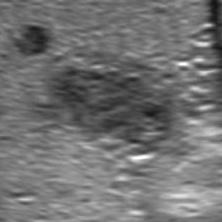
\includegraphics[width=.24\linewidth]{../fig/hemangioma.png} \label{fig:hemangioma}}
                \subfloat[Meta(転移性肝癌)]{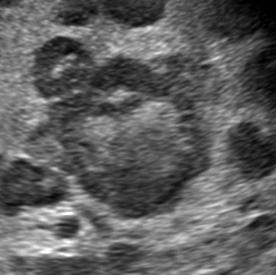
\includegraphics[width=.24\linewidth]{../fig/meta.png} \label{fig:meta}}
                \caption{症状毎における腫瘍の超音波画像}
            \end{figure}
            \begin{itemize}
                \item cyst(単純嚢胞) (\Fref{cyst})
                \begin{itemize}
                    \item 液体が貯留されている状態の良性腫瘍
                    \item 症状がでないことが多いため大きな腫瘍になって発見されることが多い
                    \item 嚢胞の内腔に向けて増殖するため転移することは少ない
                \end{itemize}
                \item HCC(肝細胞癌) (\Fref{hcc})
                \begin{itemize}
                    \item 肝臓にできる\textcolor{red}{悪性腫瘍}の中で最も多いと言われている
                    \item 約90\%がウイルス感染症が原因
                    \begin{itemize}
                        \item B型肝炎ウイルス(HBV)が約20\%
                        \item C型肝炎ウイルス(HCV)が約70\%
                    \end{itemize}
                \end{itemize}
                \item hemangioma(血管腫) (\Fref{hemangioma})
                \begin{itemize}
                    \item 肝臓にできる良性腫瘍の中で最も多い
                    \item 女性ホルモンが原因で女性が罹患しやすいと言われているが詳しくは解明されていない
                    \item 血管が無数に絡み合うことによって出来た血管の塊であることから血流が遅いという特徴がある
                    \item 他の臓器に浸潤したり転移することは無いと言われている
                \end{itemize}
                \item Meta(転移性肝癌) (\Fref{meta})
                \begin{itemize}
                    \item 門脈を介して大腸癌などの消化器癌から転移する割合が多い\textcolor{red}{悪性腫瘍}
                    \item 類似したエコーパターンをもつ腫瘤が多発してみられることが多い
                \end{itemize}
            \end{itemize}
        \end{itemize}

        \begin{itemize}
            \item データクレンジング
            \begin{enumerate}
                \item $400 \times 400$ 以下の画像の除外
                \item Perceptual Hashを利用した類似画像の除外
                \item 青色や黄色のスケールの除去
            \end{enumerate}

            \item 提供されているデータをCOCODatasetの形式に変換
            \begin{itemize}
                \item train data : test data : val data = 67122 : 8390 : 8391
                \item 見やすいようにインデントしたファイル\footnote{\url{//aka/work/hara.e/AMED/lib/dataset/annotations/train_large.json}など}も作成
            \end{itemize}

\clearpage

            \item 1クラスと4クラス検出の学習結果
            \begin{itemize}
                \item 評価指標の値を算出する為の条件
                \begin{itemize}
                    \item IoUのしきい値は0.25
                    \item 信頼度のしきい値は0.00から1.00まで0.05区切りでF1値が最大となる値
                    \begin{itemize}
                        \item YOLOX: 0.35
                        \item CenterNet: 0.30
                    \end{itemize}
                    \item 腫瘍に複数の予測がかかった時
                    \begin{itemize}
                        \item NMSで統合されていなくても正検出を1と扱う
                        \item 異なるクラスが予測された場合は信頼度が最大となる予測を検出として扱う
                    \end{itemize}
                \end{itemize}
            \end{itemize}

            \begin{figure}[h]
                \centering
                \subfloat[YOLOX\cite{yolox}での4クラス検出結果]{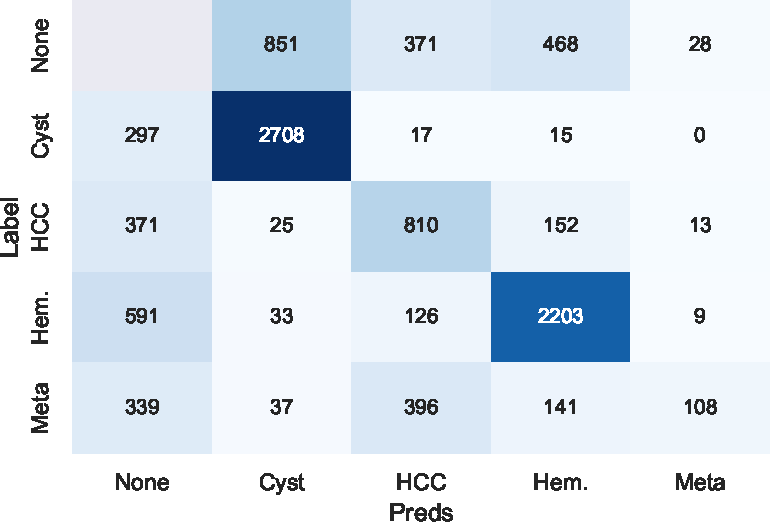
\includegraphics[width=.49\linewidth]{../fig/heatmap_yolox.pdf} \label{fig:heatmap_yolox}}
                \subfloat[CenterNet\cite{centernet}での4クラス検出結果]{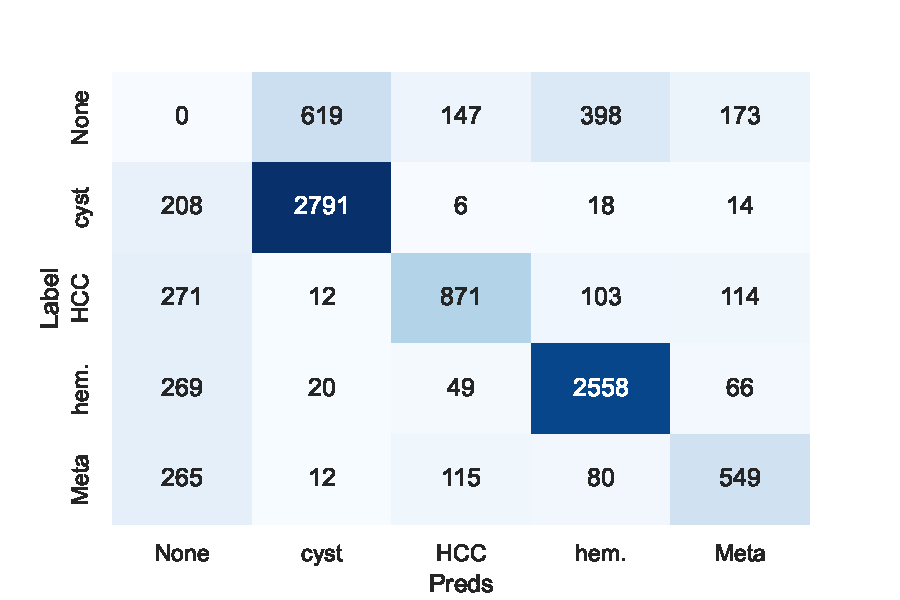
\includegraphics[width=.49\linewidth]{../fig/heatmap_center.pdf} \label{fig:heatmap_center}}
                \caption{YOLOX\cite{yolox}とCenterNet\cite{centernet}での4クラス検出した時の混同行列}
            \end{figure}

            \begin{table}[h]
                \centering
                \caption{1クラス検出と4クラス検出の学習で得られた精度}
                \label{tab:compare_models}
                \begin{tabular}{cccccc|ccc|ccc}
                    & & & & & & & IoU & & & area & \\
                    model & backbone & classes & epoch & size & batch\_size & mAP & AP$_{50}$ & AP$_{75}$ & AP$_S$ & AP$_M$ & AP$_L$ \\ \hline
                    \multirow{2}{*}{YOLOX\cite{yolox}} & \multirow{2}{*}{DarkNet} & 1 & \multirow{2}{*}{300} & \multirow{2}{*}{512} & \multirow{2}{*}{64} & 0.519 & 0.839 & 0.558 & - & 0.639 & 0.631 \\
                    &  & 4 &  &  &  & 0.279 & 0.526 & 0.248 & - & 0.221 & 0.288 \\ \hline
                    CenterNet\cite{centernet} & ResNet18 & 4 & 300 & 512 & 16 & 0.344 & 0.639 & 0.332 & - & 0.347 & 0.326
                \end{tabular}
            \end{table}

            \begin{table}[!h]
                \centering
                \caption{YOLOX\cite{yolox}で4クラス検出を行った時の評価指標毎の値}
                \label{tab:metric_yolox}
                \begin{tabular}{c|ccc|ccc}
                    Diagnosis & データ総数 & 過検出数 & 未検出数 & precision & recall & f1-score \\ \hline
                    cyst & 3037 & 851 & 297 & 0.7411 & 0.8917 & 0.8094 \\
                    HCC & 1371 & 371 & 371 & 0.4709 & 0.5908 & 0.5241 \\
                    hemangioma & 2962 & 468 & 591 & 0.7395 & 0.7438 & 0.7416 \\
                    Meta & 1021 & 28 & 339 & 0.6855 & 0.1058 & 0.1832 \\ \hline
                    合計 & 8391 & 1718 & 1598 & 0.6588 & 0.5830 & 0.5646
                \end{tabular}
            \end{table}

            \begin{table}[!h]
                \centering
                \caption{CenterNet\cite{centernet}で4クラス検出を行った時の評価指標毎の値}
                \label{tab:metric_center}
                \begin{tabular}{c|ccc|ccc}
                    Diagnosis & データ総数 & 過検出数 & 未検出数 & precision & recall & f1-score \\ \hline
                    cyst & 3037 & 619 & 208 & 0.8080 & 0.9190 & 0.8600 \\
                    HCC & 1371 & 147 & 271 & 0.7332 & 0.6353 & 0.6807 \\
                    hemangioma & 398 & 269 & 235 & 0.8103 & 0.8636 & 0.8361 \\
                    Meta & 1021 & 173 & 265 & 0.6339 & 0.5377 & 0.5669 \\ \hline
                    合計 & 8391 & 1208 & 979 & 0.7377 & 0.7389 & 0.7359
                \end{tabular}
            \end{table}

            \item 実験で用いるSimSiam\cite{simsiam}のプログラムを書いた
            \begin{itemize}
                \item 元論文のプログラムではbackboneのfc層しか用いられていなかった
                \item (自分の書いたプログラムではないからかもしれないが)汚くて使いにくかった
            \end{itemize}
        \end{itemize}

\clearpage

    \section{前回のGMからの進捗}
        \begin{itemize}
            \item SimSiam\cite{simsiam}で距離学習後に重みを全て固定したbackboneを用いて学習させたCenterNet\cite{centernet}と段階的にbackboneの重みを解除させながら学習させたCenterNet\cite{centernet}の2パターンで4クラス検出を行った

            \begin{figure}[!h]
                \centering
                \subfloat[腫瘍毎の特徴を学習するモデル]{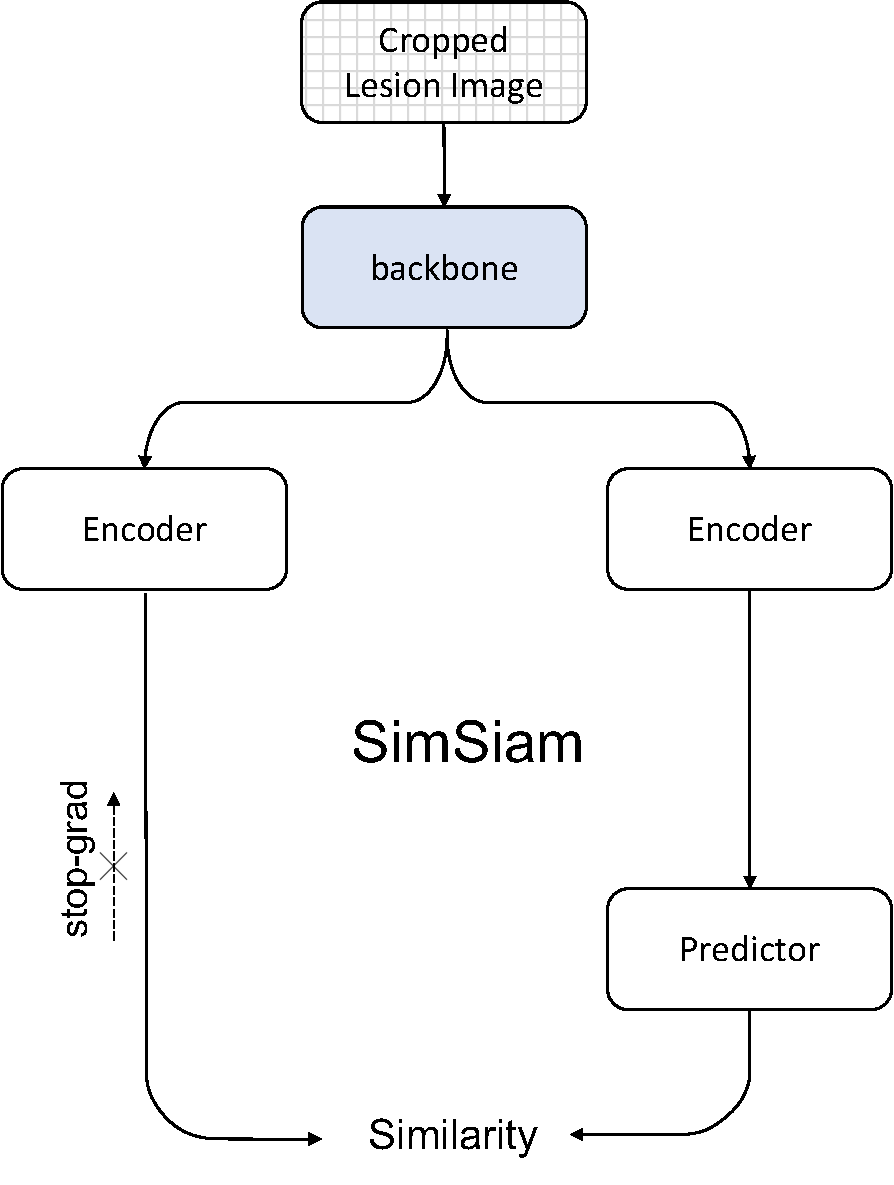
\includegraphics[width=.332\linewidth]{../fig/simsiam.pdf} \label{fig:simsiam}}
                \subfloat[学習及び推論に用いるCenterNet\cite{centernet}の概要]{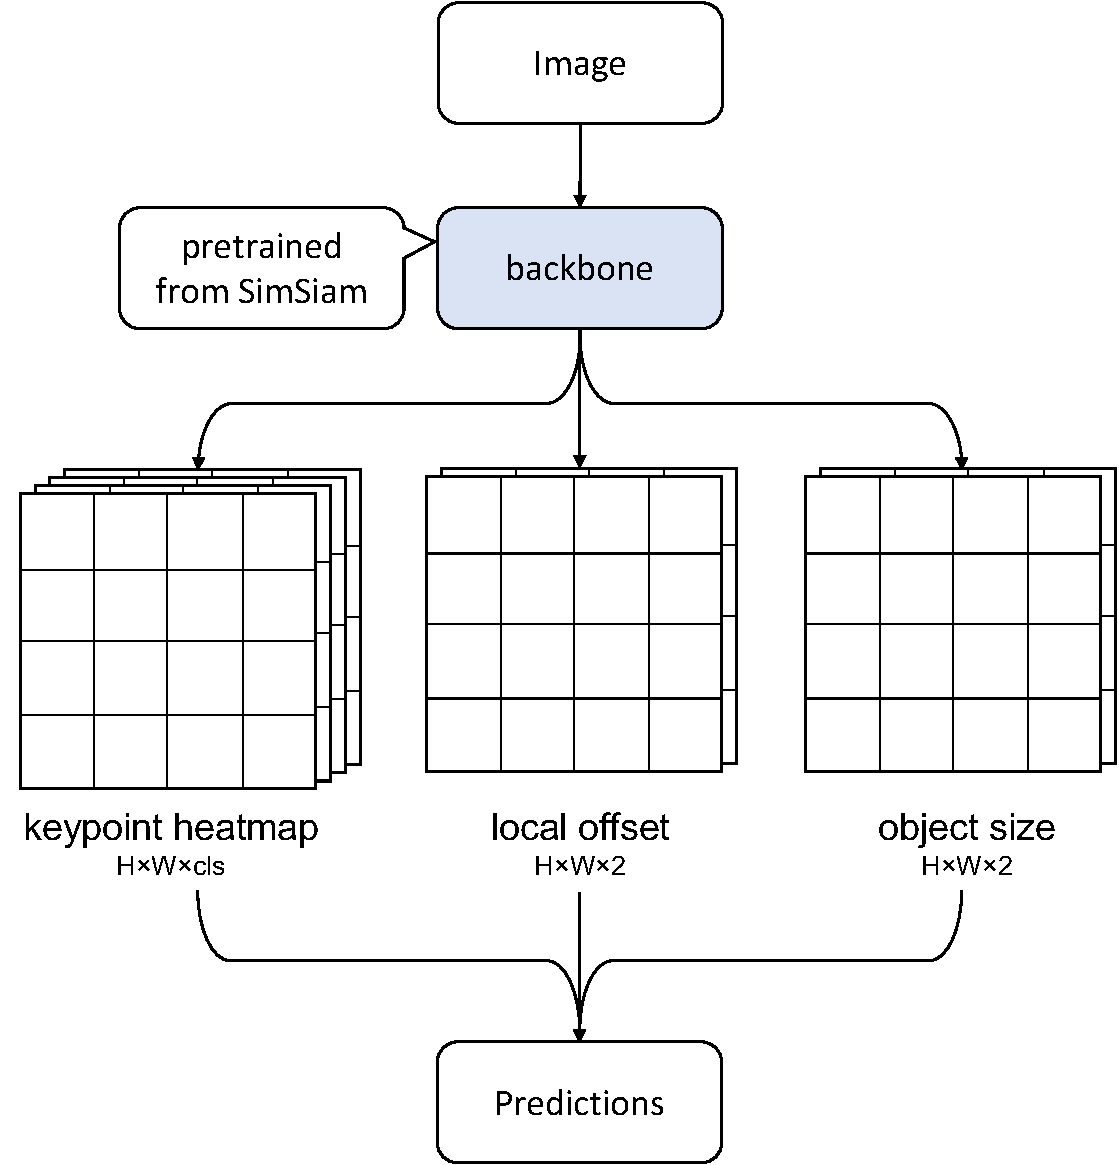
\includegraphics[width=.54\linewidth]{../fig/centernet.pdf} \label{fig:centernet}}
                \caption{実験で使用したモデル}
            \end{figure}

            \begin{figure}[!h]
                \centering
                \subfloat[backboneの重みを全て固定したモデルでの混同行列]{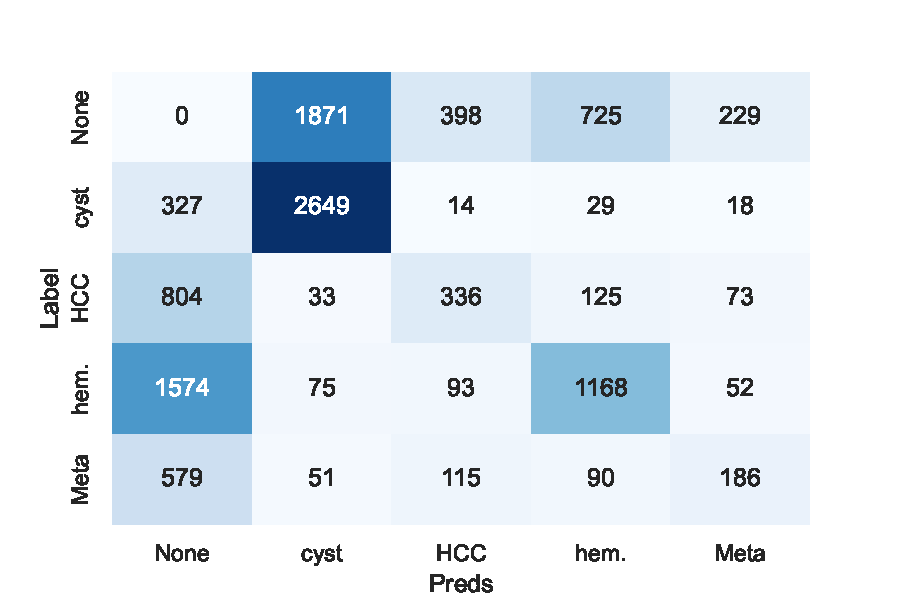
\includegraphics[width=.49\linewidth]{../fig/heatmap_centernet_fix.pdf} \label{fig:heatmap_model_fix}}
                \subfloat[段階的にbackboneの重みを解除したモデルでの混同行列]{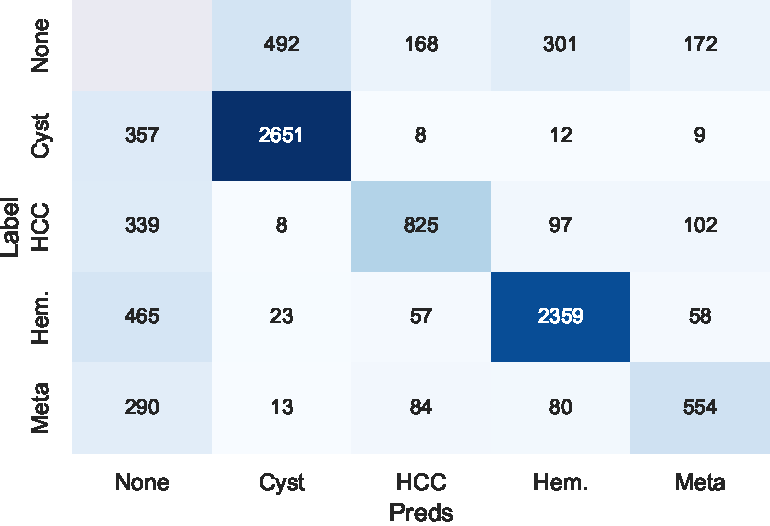
\includegraphics[width=.49\linewidth]{../fig/heatmap_centernet_stepwise2.pdf} \label{fig:heatmap_model_stepwise}}
                \caption{実験で使用したモデルでの検出と分類の結果}
            \end{figure}

            % conf = 0.20
            % \begin{table}[!h]
            %     \centering
            %     \caption{SimSiam\cite{simsiam}で距離学習後に重みを固定してCenterNet\cite{centernet}で4クラス検出を行った時の評価指標毎の値}
            %     \label{tab:metric_center_flex}
            %     \begin{tabular}{c|ccc|ccc}
            %         Diagnosis & データ総数 & 過検出数 & 未検出数 & precision & recall & f1-score \\ \hline
            %         cyst & 3037 & 1871 & 327 & 0.5661 & 0.8722 & 0.6866 \\
            %         HCC & 1371 & 398 & 804 & 0.3513 & 0.2451 & 0.2888 \\
            %         hemangioma & 398 & 725 & 1574 & 0.5466 & 0.3943 & 0.4581 \\
            %         Meta & 1021 & 229 & 579 & 0.3333 & 0.1822 & 0.2356 \\ \hline
            %         合計 & 8391 & 3223 & 3284 & 0.4494 & 0.4235 & 0.4173
            %     \end{tabular}
            % \end{table}

            % conf = 0.40
            \begin{table}[!h]
                \centering
                \caption{SimSiam\cite{simsiam}で距離学習後に段階的にbackboneの重みを解除したモデルでの評価指標毎の値}
                \label{tab:metric_center_stepwise}
                \begin{tabular}{c|ccc|ccc}
                    Diagnosis & データ総数 & 過検出数 & 未検出数 & precision & recall & f1-score \\ \hline
                    cyst & 3037 & 492 & 357 & 0.8318 & 0.8729 & 0.8519 \\
                    HCC & 1371 & 168 & 339 & 0.7224 & 0.6013 & 0.6566 \\
                    hemangioma & 398 & 301 & 465 & 0.8280 & 0.7964 & 0.8119 \\
                    Meta & 1021 & 172 & 290 & 0.6190 & 0.5426 & 0.5783 \\ \hline
                    合計 & 8391 & 1133 & 1451 & 0.7503 & 0.7034 & 0.7247
                \end{tabular}
            \end{table}

            \item 考察 (\Fref{heatmap_center}と\Fref{heatmap_model_stepwise}の比較)
            \begin{itemize}
                \item 全体的に分類精度が向上している
                \begin{itemize}
                    \item 特にMetaの分類が向上している
                    \item 分類に有効な特徴量をSimSiam\cite{simsiam}で学習できている症状もある
                    \item 検出の精度は落ちているところは問題
                    \begin{itemize}
                        \item \Fref{heatmap_model_stepwise}では信頼度の値を0.40としているからRecallが低くなっている
                    \end{itemize}
                \end{itemize}
            \end{itemize}
            \item COCOAPI (validationデータ) での結果まとめ

            \begin{table}[h]
                \centering
                \caption{1クラス検出と4クラス検出の学習で得られた精度}
                \label{tab:compare_models_sum}
                \begin{tabular}{cccccc|ccc|ccc}
                    & & & & & & & IoU & & & area & \\
                    model & backbone & weights & classes & epoch & size & mAP & AP$_{50}$ & AP$_{75}$ & AP$_S$ & AP$_M$ & AP$_L$ \\ \hline
                    \multirow{2}{*}{YOLOX\cite{yolox}} & \multirow{2}{*}{DarkNet} & \multirow{2}{*}{flex} & 1 & \multirow{2}{*}{300} & \multirow{2}{*}{512} & 0.519 & 0.839 & 0.558 & - & 0.639 & 0.631 \\
                    &  &  & 4 &  &  & 0.279 & 0.526 & 0.248 & - & 0.221 & 0.288 \\ \hline
                    \multirow{3}{*}{CenterNet\cite{centernet}} & \multirow{3}{*}{ResNet18} & flex & \multirow{3}{*}{4} & \multirow{3}{*}{300} & \multirow{3}{*}{512} & 0.344 & 0.639 & 0.332 & - & 0.347 & 0.326 \\
                    &  & fix &  &  &  & 0.150 & 0.309 & 0.127 & - & 0.119 & 0.161 \\
                    &  & stepwise &  &  &  & 0.303 & 0.568 & 0.286 & - & 0.295 & 0.309 \\
                \end{tabular}
            \end{table}
            \item CenterNetのプログラムを実装\footnote{\href{https://github.com/open-mmlab/mmdetection}{mmdetection}参考}
            \begin{itemize}
                \item モデル
                \item loss
                \item decoder
            \end{itemize}
        \end{itemize}

    \section{今後の課題\&スケジュール}
        \begin{itemize}
            \item 7/19までに
            \begin{itemize}
                \item IWAIT2023に出すabstractの内容相談
                \begin{itemize}
                    \item まだWEBサイトが公開されていなくて締め切りがわからない
                \end{itemize}
            \end{itemize}
        \end{itemize}

    \begin{thebibliography}{9}
        \bibitem{double_descent} Anonymous authors. \href{https://openreview.net/attachment?id=B1g5sA4twr&name=original_pdf}{DEEP DOUBLE DESCENT: WHERE BIGGER MODELS AND MORE DATA HURT} ICLR 2020, 2020.
        \bibitem{yolox} Zheng Ge, Songtao Liu, Feng Wang, Zeming Li, and Jian Sun. \href{https://arxiv.org/pdf/2107.08430.pdf}{YOLOX: Exceeding YOLO Series in 2021}, 2021.
        \bibitem{simclr} Ting Chen, Simon Kornblith, Mohammad Norouzi, Geoffrey Hinton. \href{https://arxiv.org/pdf/2002.05709.pdf}{A Simple Framework for Contrastive Learning of Visual Representations}, 2020.
        \bibitem{centernet} Xingyi Zhou, Dequan Wang, Philipp Krähenbühl.
        \href{https://arxiv.org/pdf/1904.07850.pdf}{Objects as Points}, 2019.
        \bibitem{simsiam} Xinlei Chen, Kaiming He. \href{https://arxiv.org/pdf/2011.10566.pdf}{Exploring Simple Siamese Representation Learning}, 2020.
    \end{thebibliography}
\end{document}
